% !TEX root = illustrator_submission.tex

\section{Performance}
\label{sec:performance}

We benchmarked our GPU-accelerated rendering mode against
\AGM/'s CPU-based renderer on six \Illustrator/
documents pictured in Figure \ref{fig:scenes}.  We selected these
scenes for their availability, artistic content, and complexity.
Table~\ref{table:scene-metrics} quantitatively summarizes each scene's
complexity.  We consider these scenes representative of the kind of
complex artwork we wish to encourage by making its authoring more
interactive.

\begin{table*}
%\small
\centering
    \begin{tabular}{| l | r | r | r | r | r | r | c |} 
\hline
      &       & 2D Control &  Clipping & Transparent  &           & Embedded & Native \\
Scene & Paths & Points     &  Masks    & Groups       & Gradients & Images & Color Space \\ \hline \hline

\hyperref[fig:bamboo]{WF\_BambooScene}	& 84,995 & 618,926 & 32,367 & 25,614 & 126 & 0 & CMYK	\\

\hyperref[fig:whale]{whale2}	& 14,403 & 481,928 & 14,333 & 14,313 & 0 & 0 & RGB	 \\

\hyperref[fig:archerfish]{ArcherFish}	& 11,214 & 	203,771 &  6,777 & 2,105 & 1,973 & 524 & RGB \\

\hyperref[fig:reef]{Tropical Reef}	&	1,041 & 6,698 & 0 & 0 & 291 & 0 & CMYK \\

\hyperref[fig:blue-mirror]{BlueMirror}	& 132,138 & 1,685,979	& 66,803 & 66,792 & 0 & 0 & RGB \\

%\hyperref[fig:beer-glass]{Beer-Glass}	&	13,151 & 141,075 & 6,579 & 6,572 & 0 & 0 & CMYK \\

%\hyperref[fig:carrot-tree]{Carrot Tree} 	& 13,998 & 129,529 & 3,672 & 3,362 & 194 & 3 & CMYK	\\

%\hyperref[fig:crowd]{Crowd (1)} 	&	93,599 & 2,627,594 & 41,941 & 41,880 & 0 & 1 & CMYK \\

\hyperref[fig:big-blend]{bigblend2} 	&	9,428 & 92,645 & 2,531 & 1,457 & 1,096 & 1 & CMYK \\

    \hline
    \end{tabular}

\caption{Scene complexity metrics.}
\label{table:scene-metrics}

\end{table*}

\begin{figure}
\centering
\subfigure[WF\_BambooScene.ai]{
   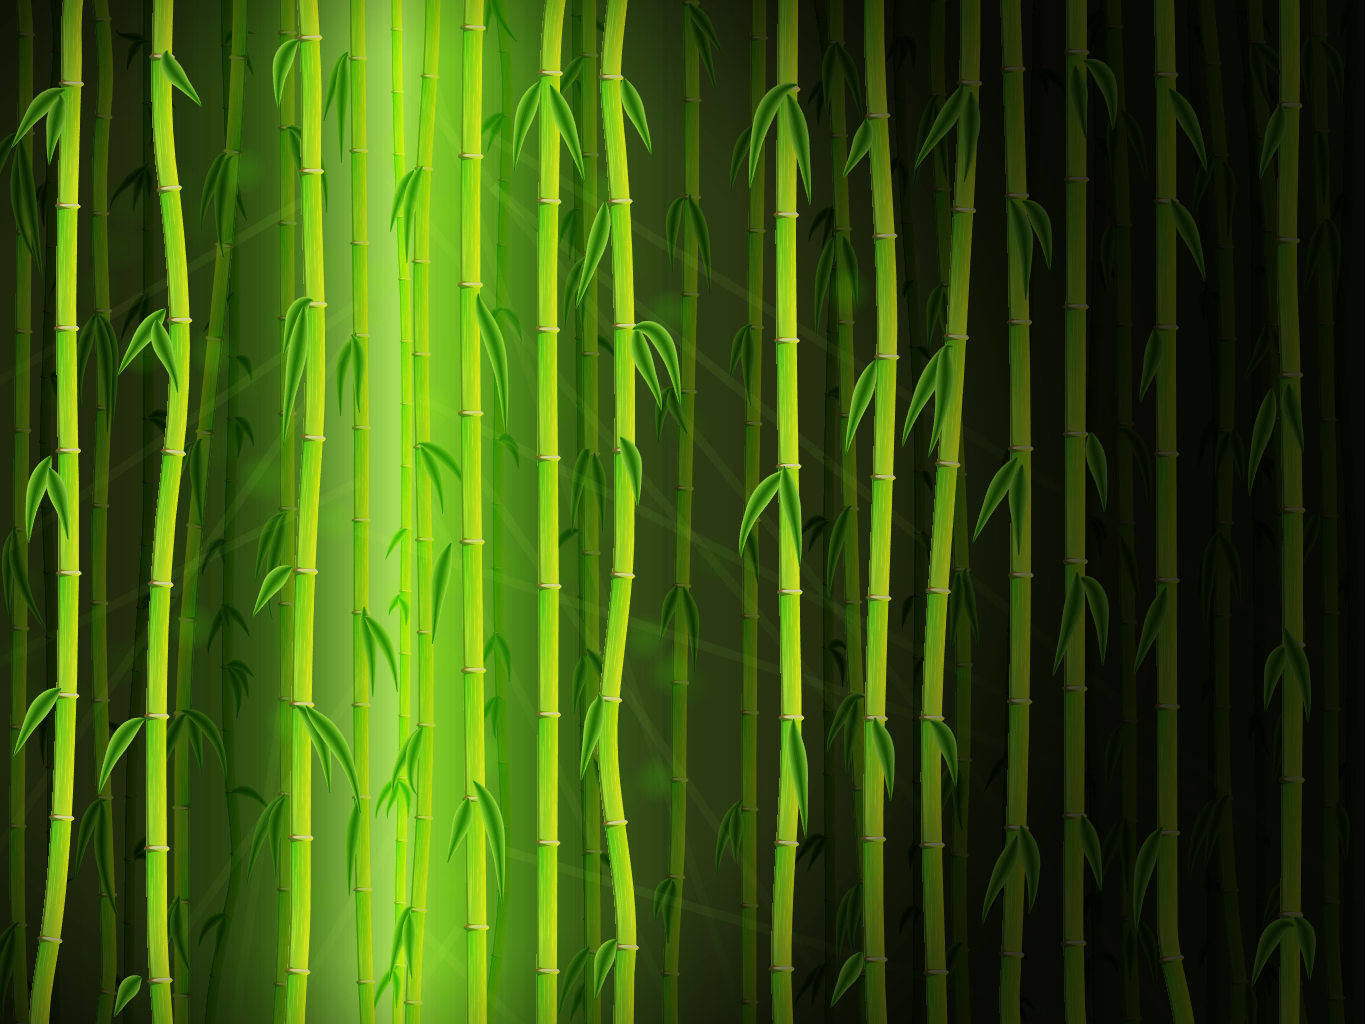
\includegraphics[height=1.4in] {benchmarks/images/fig_bamboo.png}
   \label{fig:bamboo}
 }
 %\qquad
 \\%
 \subfigure[archerfish.ai]{
   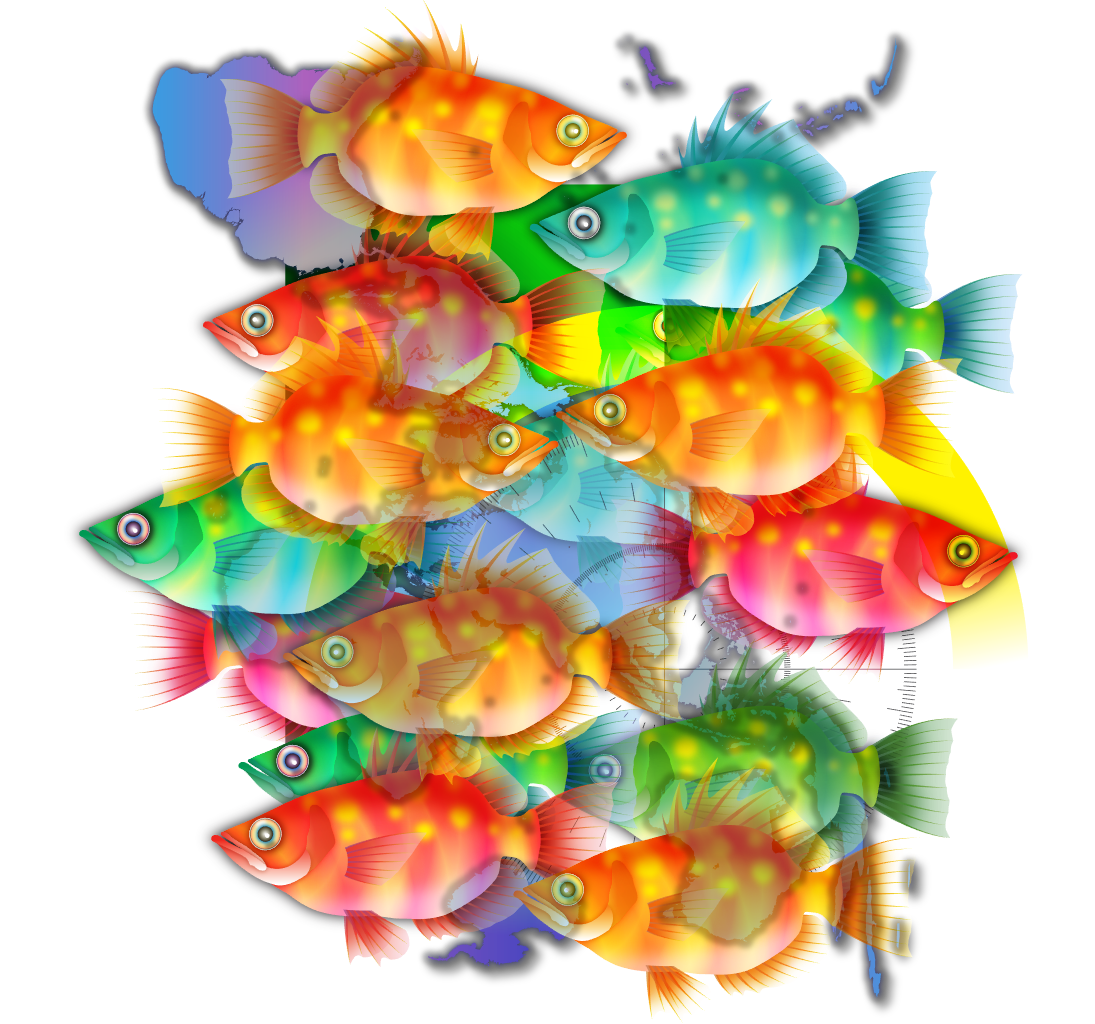
\includegraphics[height=1.62in] {benchmarks/images/fig_archerfish.png}
   \label{fig:archerfish}
 }
 \qquad
 \subfigure[Blue Mirror.ai]{
   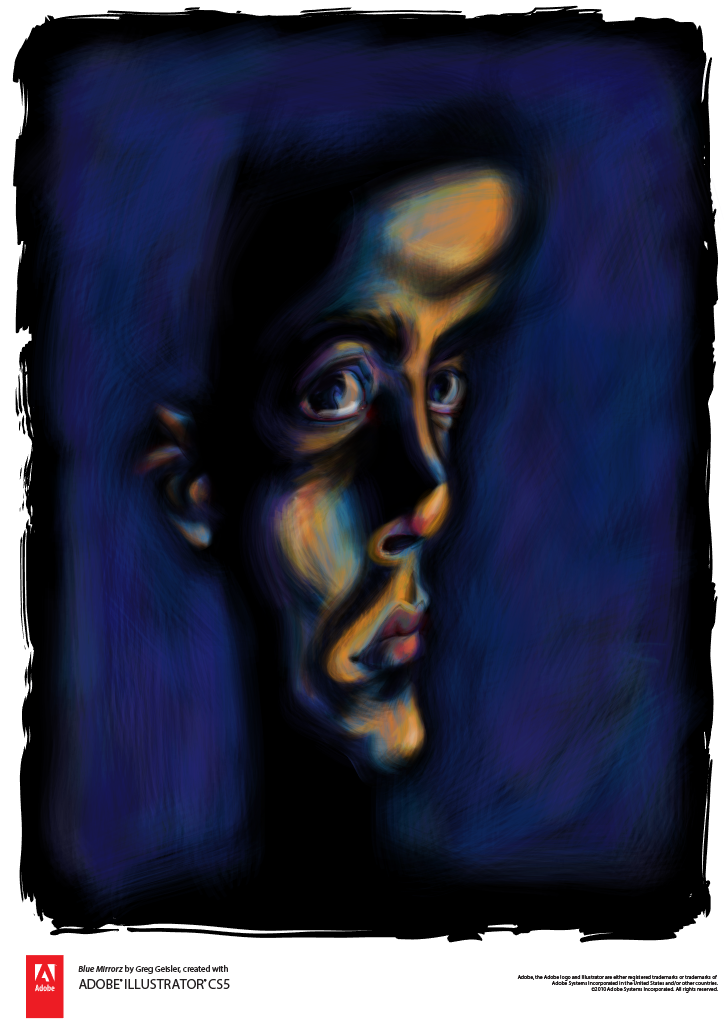
\includegraphics[height=1.62in] {benchmarks/images/fig_blue_mirror.png}
   \label{fig:blue-mirror}
 }\\%
 \subfigure[whale2.ai]{
   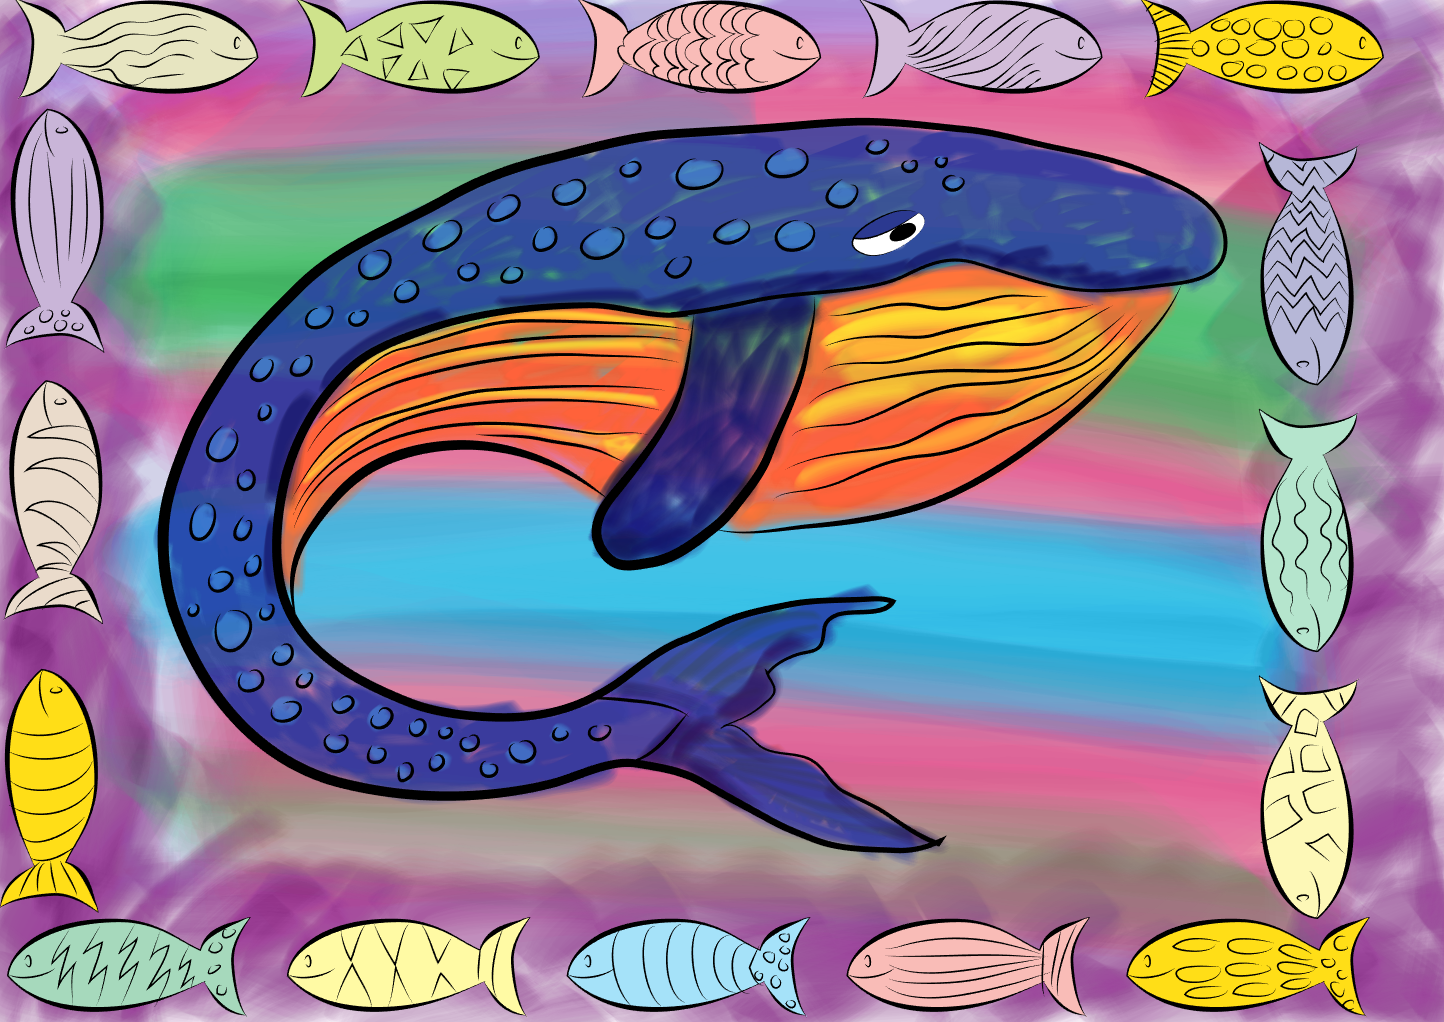
\includegraphics[height=1.4in] {benchmarks/images/fig_whale.png}
   \label{fig:whale}
 }
 \\
 %\subfigure[Beer-Glass.ai]{
 %  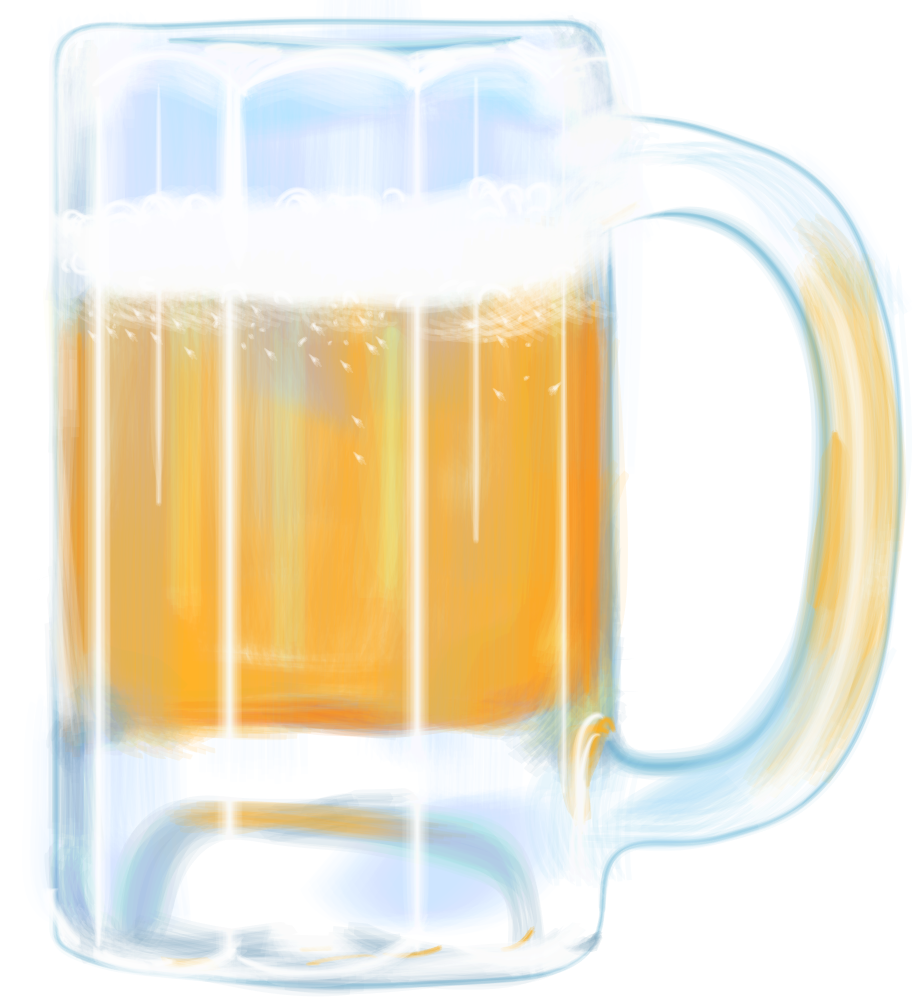
\includegraphics[width=1.2in] {benchmarks/images/fig_beer_glass.png}
 %  \label{fig:beer-glass}
 %}\qquad%
 %\subfigure[Carrot Tree Restaurant.ai]{
 %  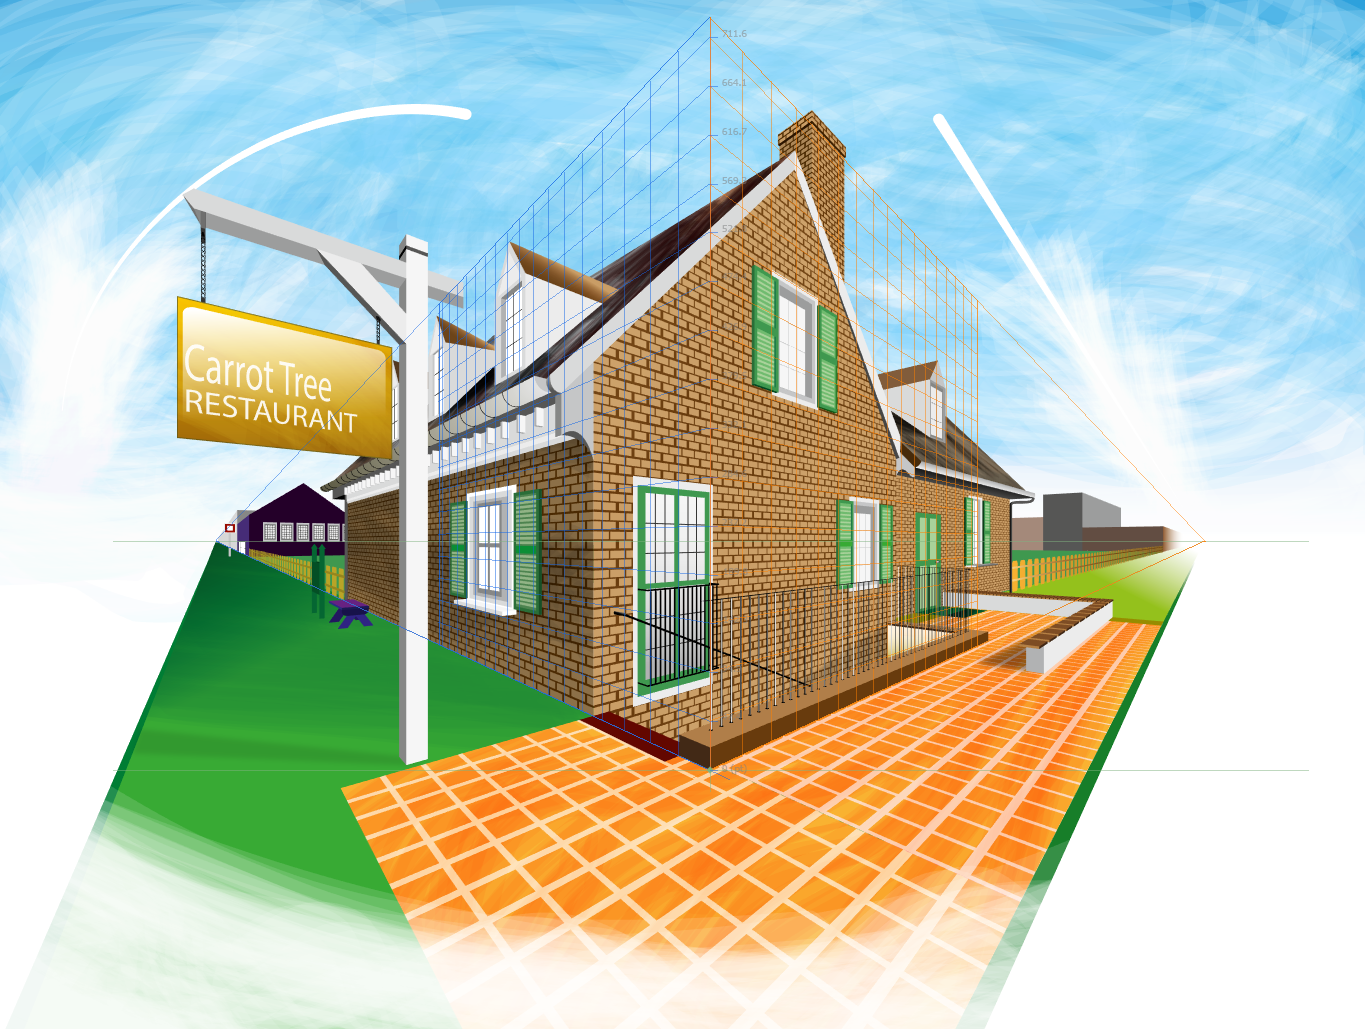
\includegraphics[width=1.6in] {benchmarks/images/fig_carrot_tree.png}
 %  \label{fig:carrot-tree}
 %}\\%
 %\subfigure[Crowd (1).ai]{
 %  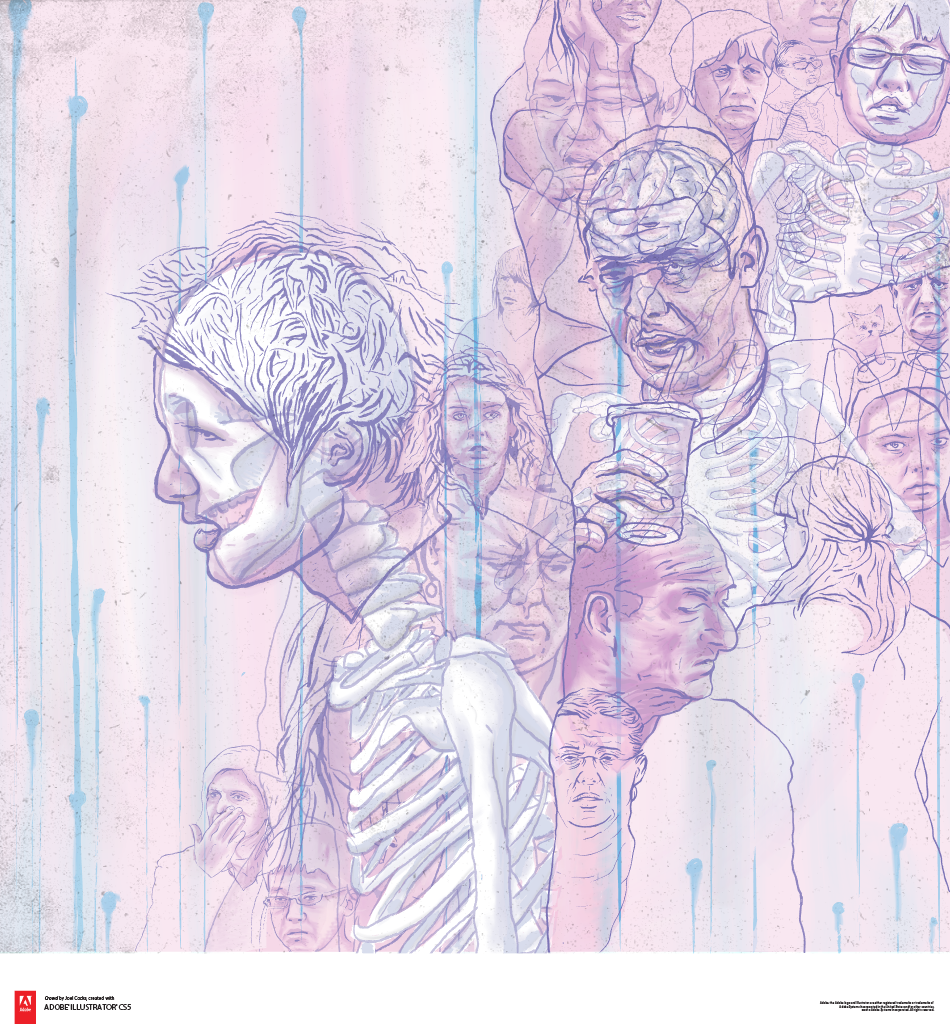
\includegraphics[width=1.1in] {benchmarks/images/fig_crowd.png}
 %  \label{fig:crowd}
 %}\qquad%
 \subfigure[Tropical Reef.ai]{
   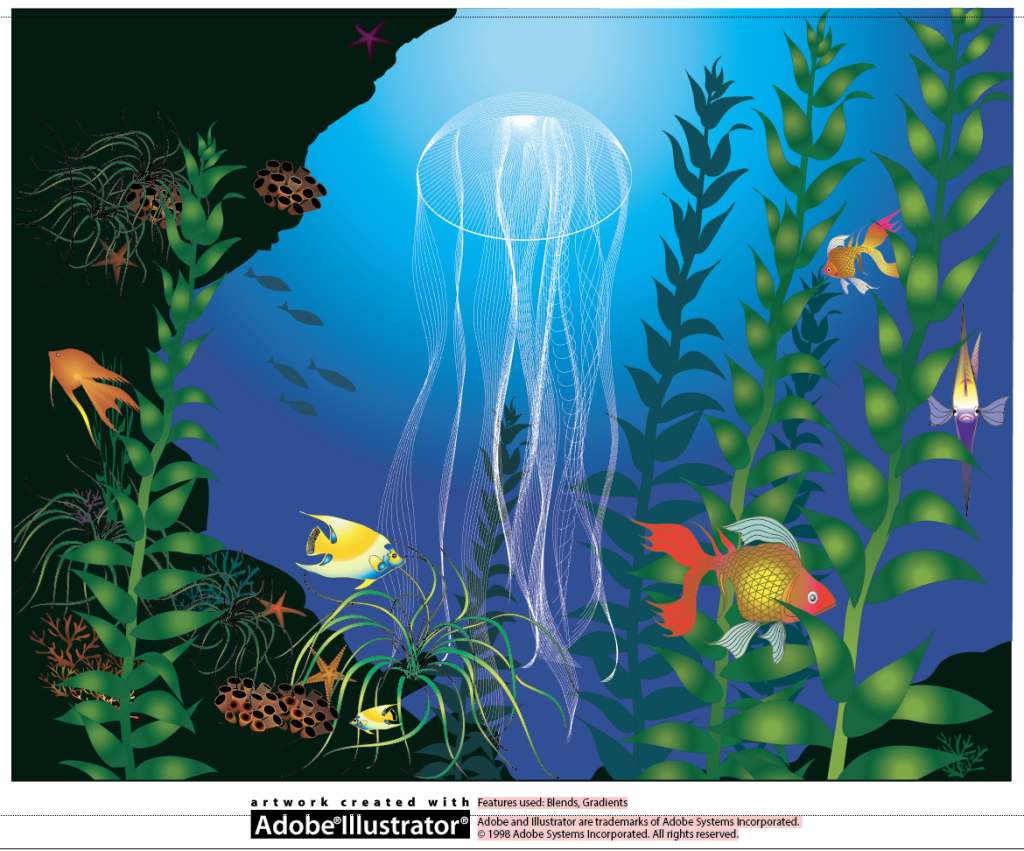
\includegraphics[height=1.4in] {benchmarks/images/ai_tropical_reef.png}
   \label{fig:reef}
 }
 \\
 %\qquad%
 \subfigure[bigBlend2.ai]{
   
\includegraphics[height=1.4in] {benchmarks/images/fig_big_blend.png}
   \label{fig:big-blend}
 }
\caption{Challenging \Illustrator/ artwork for benchmarking.}
\label{fig:scenes}
\end{figure}


\subsection{Benchmarking RGB Artwork}

Table \ref{table:rgb-scene-performance} presents our benchmarking results
for RGB color model rendering.
Our benchmarking method executes a script that zooms and pans over
the content to mimic the kind of fast view changes an artist would use
during interactive inspection of the artwork.  During the benchmark,
the \Illustrator/ application and document view are both {\em maximized}
for the most visible pixels.


Our system configuration is a Windows 7 PC with a Xeon E3-1240 V2
CPU @ 3.40GHz (4 cores), 8 GB RAM, and NVIDIA GeForce GTX 780 Ti GPU.
\AGM/'s CPU-based renderer automatically takes advantages of the CPU's
multiple cores for parallel rendering.  NVIDIA's OpenGL driver is
automatically configured for dual-core operation so the application
thread communicates OpenGL commands to a driver thread so application
and driver processing operate concurrently.  We benchmarked the 64-bit
version of the latest \Illustrator/.
\Illustrator/ always renders with 8x multisampling.


We are particularly interested in how GPU-accelerated \Illustrator/
can improve the user experience in expectation of the mass-market
adoption of {\em 4K resolution} displays so we report frame times
using Full HD resolution (1920x1080) and Ultra HD (3840x2160) monitors.
Increasing the display resolution from Full to Ultra HD increases the
geometric mean of the relative increase in CPU render time by 190\%;
but only 22\% for the GPU-accelerated transition.  We note that the
CPU rendered Ultra HD frame render times are on the order of seconds;
the GPU-accelerated frame rates are 5+ frames per second (7.9 average)
so still within what artists tolerate as interactive.

%%%% OLD TABLE
%
%\begin{table}
%    \begin{tabular}{| l | c || r | r | r |}
%    \hline
%      & Monitor HD    &        &        & \\
%Scene & Resolution & CPU ms & GPU ms & Gain \\ \hline \hline
%
%\hyperref[fig:bamboo]{WF\_Bamboo}	&	Full 	&	320	&	164	&	2.1x \\ % native CMYK
%\hspace{0.3em} \hyperref[fig:bamboo]{Scene}	&	Ultra	&	1013	&	178	&	5.6x \\ \hline
%
%\hyperref[fig:archerfish]{ArcherFish}	&	Full 	&	193	&	65	&	2.8x \\ % native RGB
%	&	Ultra	&	645	&	79	&	6.6x \\ \hline
%
%\hyperref[fig:whale]{whale2}	&	Full &	341	&	110	&	3.5x \\  % native RGB
%	&	Ultra	&	906	&	121	&	7.1x \\ \hline
%
%\hyperref[fig:blue-mirror]{BlueMirror}	&	Full &	923	&	193	&	4.2x \\  % native RGB
%	&	Ultra	&	2011	&	212	&	7.8x \\ \hline
%
%\hyperref[fig:beer-glass]{Beer-Glass}	&	Full 	&	229	&	46	&	5.3x \\  % native CMYK
%	&	Ultra	&	588	&	66	&	9.9x \\ \hline
%
%\hyperref[fig:carrot-tree]{Carrot Tree} 	&	Full 	&	130	&	35	&	3.5x \\  % native CMYK
%\hspace{0.3em} \hyperref[fig:carrot-tree]{Restaurant} &	Ultra	&	420	&	47	&	9.3x \\ \hline
%
%\hyperref[fig:crowd]{Crowd (1)} 	&	Full 	&	712	&	150	&	4.8x \\  % native CMYK
%	&	Ultra	&	1963	&	203	&	10.0x \\ \hline
%
%\hyperref[fig:big-blend]{bigblend2} 	&	Full 	&	656	&	94	&	6.2x \\  % native CMYK
%	&	Ultra	&	2361	&	109	&	16.7x \\ \hline
%
%    \hline
%    \end{tabular}
%
%\caption{Average frame time in milliseconds rendering complex art scenes at varying zooms and panning, comparing the
%existing CPU rendering mode to our new GPU-accelerated mode.  {\em Gain} is the geometric mean of the speedup of
%GPU over the CPU mode for corresponding benchmark frames.
%}
%\label{table:rgb-scene-performance}
%
%\end{table}

\begin{table}
    \begin{tabular}{| l | c || r | r | r |}
    \hline
RGB mode & Monitor HD    &        &        & \\
Scene & Resolution & CPU ms & GPU ms & Gain \\ \hline \hline

\hyperref[fig:bamboo]{WF\_Bamboo}	&	Full 	&  320	&	174	&	3.53x \\ % native CMYK
\hspace{0.3em} \hyperref[fig:bamboo]{Scene}	&	Ultra	&1071	&	219	&	5.23x	\\ \hline

%\hyperref[fig:carrot-tree]{Carrot Tree} 	&	Full 	&104	&	22	&	4.54x	\\  % native CMYK
%\hspace{0.3em} \hyperref[fig:carrot-tree]{Restaurant} &	Ultra	&292	&	38	&	7.49x	\\ \hline

\hyperref[fig:whale]{whale2}	&	Full &336	&	37	&	8.41x	\\  % native RGB
	&	Ultra	&1015	&	129	&	8.02x	\\ \hline

\hyperref[fig:archerfish]{ArcherFish}	&	Full 	&259	&	28	&	9.04x	\\ % native RGB
	&	Ultra	&979	&	100	&	9.59x	\\ \hline

%\hyperref[fig:beer-glass]{Beer-Glass}	&	Full 	&291	&	24	&	9.29x	\\  % native CMYK
%	&	Ultra	&562	&	80	&	7.38x	\\ \hline

\hyperref[fig:reef]{Tropical Reef}	&	Full 	&64	&	20	&	3.36x	\\  % native CMYK
	&	Ultra	&179	&	30	&	6.28x	\\ \hline

\hyperref[fig:blue-mirror]{BlueMirror}	&	Full &1209	&	100	&	11.39x	\\  % native RGB
	&	Ultra	&2971	&	279	&	10.98x	\\ \hline

%\hyperref[fig:crowd]{Crowd (1)} 	&	Full 	&636	&	49	&	14.31x	\\  % native CMYK
%	&	Ultra	&1875	&	149	&	14.43x	\\ \hline

\hyperref[fig:big-blend]{bigblend2} 	&	Full 	&828	&	44	&	14.38x	\\  % native CMYK
	&	Ultra	&3211	&	142	&	17.54x	\\ \hline

    \hline
    \end{tabular}

\caption{Average frame time in milliseconds rendering complex art
scenes in RGB document mode (CMYK artwork is forced to RGB) at varying
zooms and panning, comparing the existing CPU rendering mode to our new
GPU-accelerated mode.  {\em Gain} is the geometric mean of the speedup
of GPU over the CPU mode for corresponding benchmark frames.
}
\label{table:rgb-scene-performance}

\end{table}

\begin{table}
    \begin{tabular}{| l | c || r | r | r |}
    \hline
CMYK mode & Monitor HD    &        &        & \\
Scene & Resolution & CPU ms & GPU ms & Gain \\ \hline \hline

\hyperref[fig:bamboo]{WF\_Bamboo}	&	Full 	&  392	&	405	&	1.34x \\ % native CMYK
\hspace{0.3em} \hyperref[fig:bamboo]{Scene}	&	Ultra	&1520	&	630	&	2.37x	\\ \hline

\hyperref[fig:reef]{Tropical Reef}	&	Full 	&99	&	22	&	4.80	\\  % native CMYK
	&	Ultra	&311	&	38	&	9.28x	\\ \hline

\hyperref[fig:big-blend]{bigblend2} 	&	Full 	&861	&	111	&	6.73x	\\  % native CMYK
	&	Ultra	&3542	&	381	&	10.55x	\\ \hline

    \hline
    \end{tabular}

\caption{Average frame time in milliseconds rendering complex CMYK art
scenes at varying
zooms and panning, comparing the existing CPU rendering mode to our new
GPU-accelerated mode.  {\em Gain} is the geometric mean of the speedup
of GPU over the CPU mode for corresponding benchmark frames.
}
\label{table:cmyk-scene-performance}

\end{table}

\subsection{Benchmarking CMYK Artwork}

Table~\ref{table:cmyk-scene-performance} presents CMYK benchmarking results for the three ``native CMYK'' scenes
listed in Table~\ref{table:scene-metrics}.
Whereas the benchmarking of these scenes in Table~\ref{table:rgb-scene-performance} forced the scenes
be converted to RGB, Table~\ref{table:cmyk-scene-performance} benchmarks these scenes in their
native CMYK color space by rendering with a CMYK framebuffer.

The WF\_BambooScene scene is included specifically because it demonstrates rather poor GPU rendering performance,
particularly when rendered in the scene's native CMYK color space.
The WF\_BambooScene scene is an example of a scene constructed in ways that stress GPU rendering with poor results---though the scene is quite challenging for CPU rendering too!
First the scene itself has a large number of paths,
a variety of blend modes, and uses knockout.  The scene already has a large number of transparency groups, but many become
non-trivial groups when used with non-{\em Normal} blend modes and knock-out.
Recall \NVbea/ limitations that make blend modes overly expensive in CMYK rendering (Section \ref{sec:tweaks}).
Additionally when zoomed out of the scene, there is a large number of intricate
paths placed invisibly outside the scene's framed view (this is not uncommon for artists to do as
a way of stashing fragments of artwork).  The effect is acceptable GPU-acceleration when zoomed into
the CMYK scene but worse-than-CPU-rendering performance when zoomed out.  Performance is good zoomed
in because the pathological features of the scene get view culled away.

\begin{figure}[tb]
  \center{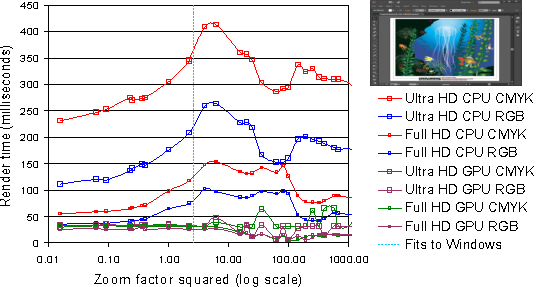
\includegraphics[width=\columnwidth]{images/illustrator_performance.pdf}}
  \caption{\label{fig:zoom-perf}
Rendering time for Tropical Reef.ai scene, comparing GPU vs. CPU, Full vs. Ultra HD, and RGB vs. CMYK at over a large range of zoom factors squared.  Dashed vertical lines indicate the zoom factor when the scene ``Fits to Window'' for Full and Ultra HD respectively.
}
\end{figure}

We now look at a more typical scene in detail.
Figure~\ref{fig:zoom-perf} graphs the render time for at a variety of zoom levels
for the (native CMYK) Tropical Reef scene.  Illustrator documents are in ``real world''
dimensions so a 100\% zoom corresponds to its printed dimensions.  We graph the zoom factor squared
(so 1 is a 100\% zoom and 4 is a 200\% zoom) because this normalizes the screen-space area of a given scene region.
The graph shows the scene rendered in
all eight combinations of CPU/GPU rendering, Full/Ultra HD resolution, and CMYK/RGB color models
over a range of zoom levels.  While the original scene is authored in CMYK, by forcing a conversion
to the RGB color mode, we can compare the relative expense of CMYK relative to RGB rendering.

While the window size in pixels is constant at either Full or Ultra
HD resolution, the render time is not stable at increasing zoom levels
because many objects can be culled from the scene as the zoom increases
while also small objects become large and hence more expensive to draw.
This factor affects both the CPU and GPU render times but in different
ways we now explore.

The CPU renderer is sensitive to having a large number of objects, and
hence active edges, to process.  Also complex shading and blending is
relatively more expensive for the CPU while shading and blending are
quite efficient for the GPU.  In contrast while the CPU's scan-line 
rasterizer is quite work-efficient and ``cache friendly'' because it operates
on just a scan-line at a time, the GPU renderer is challenged when
paths are large in screen space so the overdraw from the ``stencil'' step
becomes rasterization bound.  Lots of stencil counting that ultimately cancels to zero or
generates large winding number magnitudes create costly rasterization burdens for the GPU.
Likewise expensive quadratic discard shaders for curved stroked segments become
expensive when the stroke width is more than a fix pixels wide in screen space.

Even so, GPU performance is consistently faster than the CPU performance but subject
to more significant variations at different zoom levels.  To help quantify the relative
cost of CMYK rendering via the GPU we can compare native CMYK rendering on the GPU to
an RGB-converted version of the Tropical Reef content in Figure~\ref{fig:zoom-perf}.
RGB-converted rendering averages
36\% (Full HD) to 43\% (Ultra HD) faster than CMYK rendering with the CPU.
The GPU averages 6\% (Full HD) to 9\% (Ultra HD) faster when the
CMYK artwork is converted to RGB but these averages mask significant
variability.  So while the framebuffer memory consumption for CMYK is at least double
the storage for RGB color mode rendering, the observed performance cost is not nearly so bad
and is still much faster than CMYK rendering on the CPU.

\subsection{Comparison with Recent Work}
\label{sec:mpvg}

\cite{GanEtAl14} provides performance results for a number of SVG scenes
using a massively-parallel vector graphics (MPVG) system based on CUDA.  Table~\ref{table:mpvg}
presents a subset of their scenes most relevant to an Illustrator artist with results from our comparable PC configuration.  Our rendering performance relies on
\NVpr/ but performs markedly better than the \NVpr/ performance reported in their paper.
We attribute this to forcing use of NVIDIA's dual-core
driver and Illustrator's tuned OpenGL usage and scene traversal.
For all but two of scenes in our table, GPU-accelerated Illustrator is faster than their published results---the
exceptions are a detailed but inefficiently authored (so CPU bound) Paris map and their---arguably pathological---Contour scene.

MPVG's strengths are antialiasing quality and an ability to handle what would typically be considered
inefficiently structured scenes---strengths we readily acknowledge.
Since Illustrator supports just 8x multisampling and their reported
image resolutions are rather low, we provide ``double resolution''
rendering results as an alternative for their 32x rendering quality.

While MPVG's rendering quality and novelty of approach is impressive,
Illustrator must support the entire PDF rendering model including CMYK, blend modes,
transparency groups, etc. all while making everything editable.

\begin{table}
    \begin{tabular}{| l | l || r | r | r |}
    \hline
      &            & MPVG & MPVG & Illustrator \\
Input & Resolution & 8x & 32x & GPU 8x \\
    \hline
    \hline

Car & 1024x682 & 12.86 & 14.73 & 2.94 \\
    & 2048x1364 & & & 3.09
\\ \hline
Drops & 1024x1143 &14.28 & 18.59 & 2.29 \\
    & 2048x2286 & & & 6.21
\\ \hline
Embrace & 1024x1096 &15.50 & 19.38 &  1.69 \\
    & 2048x2192 & & & 3.63
\\ \hline
Reschart & 1024x625 &8.51 & 11.14 & 1.92 \\
    & 2048x1250 & & & 2.60
\\ \hline
Tiger & 1024x1055 &12.89 & 17.24 &  1.48 \\
    & 2048x2110 & & & 5.34
\\ \hline
Boston & 1024x917 &37.22 & 41.81 &  2.66 \\
    & 2048x1834 & & & 5.02
\\ \hline
Hawaii & 1024x844 &26.16  &29.48 &  3.83 \\
    & 2048x1688 & & & 8.75
\\ \hline
Contour & 1024x1024 &30.07 & 30.36 & 90.53 \\
    & 2048x2048 & & & 328.57
\\ \hline
Paris 50K & 1024x1024 &26.82 & 25.22 & 65.53 \\
    & 2048x2048 & & & 64.23
\\ \hline

    \end{tabular}
    \caption{Comparison of SVG content render times (in milliseconds) reported by \protect\cite{GanEtAl14} to our work with Illustrator.}
\label{table:mpvg}

\end{table}
